\section{はじめに}
\label{はじめに}

\subsection{研究背景}
\label{研究背景}
近年,Apple社のSiriなどのスマートフォン上で動作する音声エージェントサービスや,Amazon社のAlexaなどのスマートスピーカーに見られるように,ユーザの発言に対して正しい応答や人間らしい応答を返すための音声対話技術がめざましく進歩している.今後,このような対話システムは,様々な形で,私達の日常活動を支援するものと期待される.\cite{kikiyaku2012} \cite{koreisya2000}しかし,日常活動での対話は,スマートスピーカーとの対話よりも複雑であり,現在の音声対話技術でも,様々な状況においてうまく対話を継続して目的を達成するのは困難である\cite{hitask2016}.例えば対話を通した接客業務では,話し方や要望の出し方など対話相手よって様々であり,それに適切に対応する必要がある.このとき,私達人間であれば,対話相手のタイプによって話し方を切り替えて対応したり,音声だけでなく視線や表情などもうまく使って対話を継続することができるが,音声対話システムではこのような対応を取ることができない.人型ロボットは,様々なセンサを用いてユーザの音声だけでなく表情やしぐさなどを認識できたり,体を用いてジェスチャや表情など様々な表現ができる.音声対話システムよりも複雑である反面,多くの情報や多くの表現手段を用いることで,従来の対話システムとは異なる方法で対話をうまく継続を実現できる可能性がある.本研究では音声,表情,身振り,手振りなどのモダリティを用いて円滑に対話を進めるマルチモーダル音声対話システムの構築を目指す.

\subsection{研究の位置付け}
情報化社会の次に来るであろう人間と知能ロボットや情報メディアが共生する社会を実現するため,「人間機械共生社会を目指した対話知能システム学(対話知能学)」\footnote{https://www.commu-ai.org/}が文部科学省科学研究費助成事業「新学術領域研究」として2019年に創生された.対話内容を完全に理解できずとも違和感なく対話を継続できる能力を実現する「対話継続関係維持」,特定の状況において特定の目的に関して対話理解と対話生成を組み合わせた対話能力を実現する「対話理解生成」,システムが自らの行動決定モデルを構築したり相手の行動決定モデルを推定する機能を実現する「行動決定モデル推定」,実証実験を通して意図や欲求を持つロボットの人々への影響を研究,ロボット共生社会における社会規範を提案する「人間機械社会規範」の4つの軸を元に,人間と機械や情報メディアが互いの意図や欲求を推定し合いながら関わり合う社会の実現を目指す.複数の情報を統合し状況に適応的にふるまうマルチモーダル音声対話システムの構築は「対話理解生成」に相当する.
\begin{figure}[th]
    \centering
    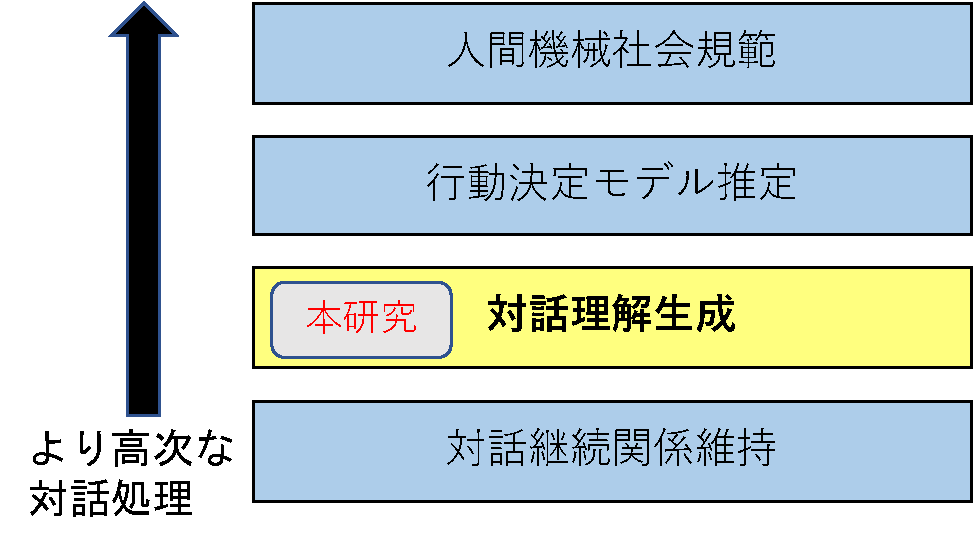
\includegraphics[scale=0.5]{pic/commuai.pdf}
    \caption{対話システム構築の位置付け}
    \label{commuai}
\end{figure}


\subsection{研究目的}
\label{研究目的}
本研究では,旅行代理店業務において,カウンターセールスを行う音声対話システムの構築を目指す.対話システムは,音声,表情,身振り,手振りなどのモダリティをもち,身体性も有する.複数のモジュールを用いてロボットの身体管理,対話管理を行うことでロボットと音声で対話実現をすることで,テキストだけの対話システムや音声だけの対話システムに比べ,ホスピタリティの高い対話を実現することを目標とする.

\subsection{本論文の構成}
\label{本論文の構成}
以下に本論文の構成を記述する.\ref{関連研究}章では,音声対話システムの関連研究について説明する. \ref{対話システムの構築}章では提案手法の概要とシステムのモジュールについて説明する.\ref{評価実験}章では対話ロボットコンペティションにおいての実験について述べる.\ref{考察}章で構築した対話システムに関する考察を行い,\ref{まとめ}章でまとめについて述べる.
